\chapter{Resultados experimentales}
\label{resultados}

En este capítulo se resumen los resultados obtenidos. Los detalles de los experimentos se pueden consultar en \autoref{anexo1}.

\section{Comparación de parámetros $G$ y $N$}
Como se explicó en el \autoref{heurístico}, el algoritmo desarrollado depende de dos parámetros: $G$, la frecuencia con la que realizamos la fase constructiva; y $N$, el número máximo de elementos que puede contener la cola de vuelos extras.

Tras realizar varias pruebas, hemos podido comprobar que, como era de esperar, los mejores resultados se obtienen con un parámetro $N$ pequeño y $G$ grande:
\begin{itemize}
	\item Un \textbf{\textit{N} pequeño} implica realizar la fase constructiva con mucha frecuencia. Esto hace que cada pocas iteraciones busquemos un intento de mejora, y por tanto en caso de no conseguir mejorar la solución actual descartaremos la cola de vuelos extras con mucha rapidez.
	
	Un $N$ pequeño también aporta más desviación a los resultados, ya que al descartar colas con mucha facilidad, hace que el problema se reinicie con más frecuencia, y por tanto tenga más aleatoriedad. 
	
	\item Un \textbf{\textit{G} grande} implica que se de más peso a las buenas soluciones que se localizaron en la cola anterior. Por tanto al tener una cola de vuelos extras de gran tamaño, permite que las buenas soluciones tengan una probabilidad mucho mayor que salir antes en el proceso aleatorio de selección de orden de los vuelos para intentar ser colocados.
\end{itemize} 

Concretamente, hemos podido comprobar mediante pruebas con diferentes parámetros que los la configuración óptima de los parámetros es la siguiente:
\begin{itemize}
	\item \textbf{N:} si es demasiado pequeño, el algoritmo no dispone de las iteraciones suficientes para tratar de obtener información relevante para futuras simulaciones, por lo que el valor óptimo del parámetro es un 5\% del total de iteraciones. De esta forma, en un ejemplo sobre el que realizamos 100 iteraciones, realizaremos la fase constructiva en 20 ocasiones. 
	\item \textbf{G:} aunque el algoritmo funciona mejor con un parámetro \textit{G} elevado, los valores óptimos se alcanzan cuando es un 50\% sobre el número total de vuelos. Por tanto si disponemos de un modelo con 100 vuelos, la cola máxima de vuelos que seleccionaremos para las siguientes iteraciones será de como mucho 50. De esta forma se evita que las iteraciones se parezcan demasiado entre si.
\end{itemize}


\section{Evolución de la función objetivo}
Como ya comentamos, con la configuración de parámetros $G$ y $N$ al descartarse muy rápido las malas combinaciones obtenemos un gran número de reseteos del problema, por lo que obtenemos una desviación alta. En la \autoref{fig: Evolucion función objetivo} se muestra la evolución del valor de la función objetivo en un ejemplo de 100 vuelos con parámetro $N=5$: 
\begin{figure}[H]
	\begin{center}
		\centering
		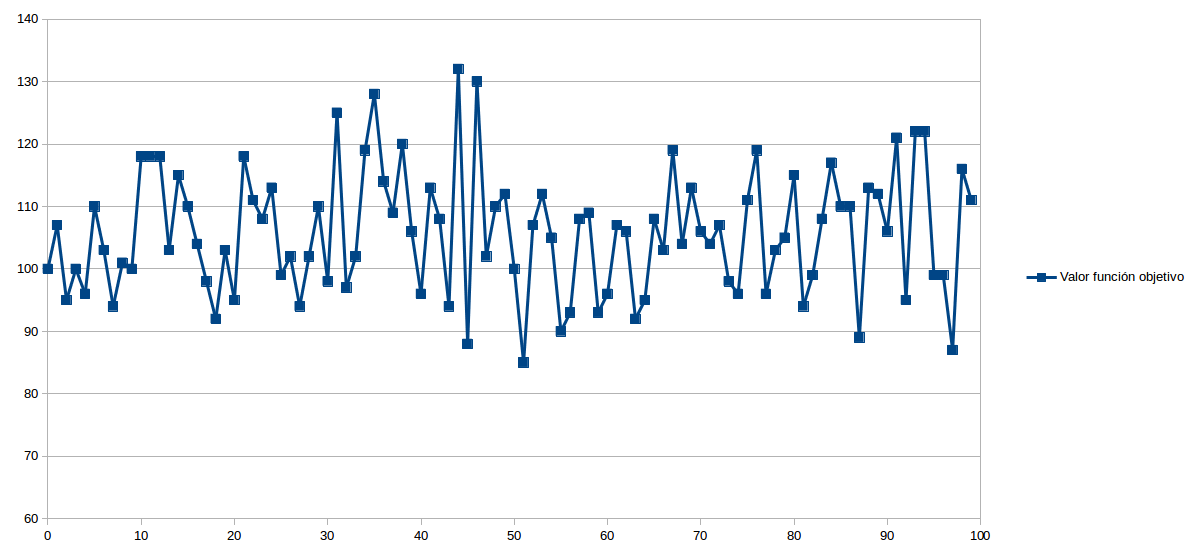
\includegraphics[width=1\textwidth]{./imagenes/resultados/evolucionFuncionObjetivo.png}
		\caption{Evolución función objetivo con $N=5$ y $G=20$ con ejemplo de 100 vuelos}
		\label{fig: Evolucion función objetivo}
	\end{center}
\end{figure}
Como se puede comprobar, en las iteraciones en las que se produce la fase de evaluación y se decide si se descarta la cola, se pueden dar importantes saltos. Por ejemplo, en la \autoref{fig: Evolucion función objetivo} se puede observar como en la iteración con $x=40$ ha habido un descarte de la cola que se había elegido en la anterior fase de mejora, ya que en la siguiente iteración ha habido una gran mejora.

Por el contrario en las iteraciones $x=60$ o $x=80$ se puede observar que no se ha descartado la cola de candidatos, ya que la mejora en la función objetivo ha sido mas leve.

\section{Resultados globales}
A continuación se muestran resumidos los resultados de las pruebas realizadas en los 3 problemas que disponíamos para probar el algoritmo. Los valores se corresponden con la simulación de 100 problemas de 100 iteraciones cada uno con los parámetros $G$ y $N$ óptimos:
\begin{table}[H]
	\centering
	\caption{Resultados pruebas 20 vuelos}
	\label{resultados 20 vuelos}
	\begin{tabular}{lllll}
		& \textbf{\% Vuelos con solución} & \textbf{Valor función objetivo} & \textbf{} & \textbf{} \\
		\textbf{Caso A} & \multicolumn{1}{c}{99.61\%} &\multicolumn{1}{c}{46.8} & &\\
		\textbf{Caso B} & \multicolumn{1}{c}{100\% }    &\multicolumn{1}{c}{47} & &\\
		\textbf{Caso C} & \multicolumn{1}{c}{100\%}    &\multicolumn{1}{c}{45} & &
	\end{tabular}
\end{table}


\begin{table}[H]
	\centering
	\caption{Resultados pruebas 100 vuelos}
	\label{resultados 100 vuelos}
	\begin{tabular}{lllll}
		& \textbf{\% Vuelos con solución} & \textbf{Valor función objetivo} & \textbf{} & \textbf{} \\
		\textbf{Caso A} & \multicolumn{1}{c}{61.69\%} &\multicolumn{1}{c}{118.57} & &\\
		\textbf{Caso B} & \multicolumn{1}{c}{93.73\%}    &\multicolumn{1}{c}{200.88} & & \\
		\textbf{Caso C} & \multicolumn{1}{c}{99.96\%}    &\multicolumn{1}{c}{217.88} & &
	\end{tabular}
\end{table}

Como se puede observar, exceptuando el caso de pruebas \textit{A} que tiene un gran número de vuelos iguales simultáneos, los resultados se mueven siempre en porcentajes mayores al 90\%.

\section{Representación gráfica}
A continuación se muestra la representación gráfica obtenida para un problema con 20 vuelos.
\begin{figure}[H]
	\begin{center}
		\centering
		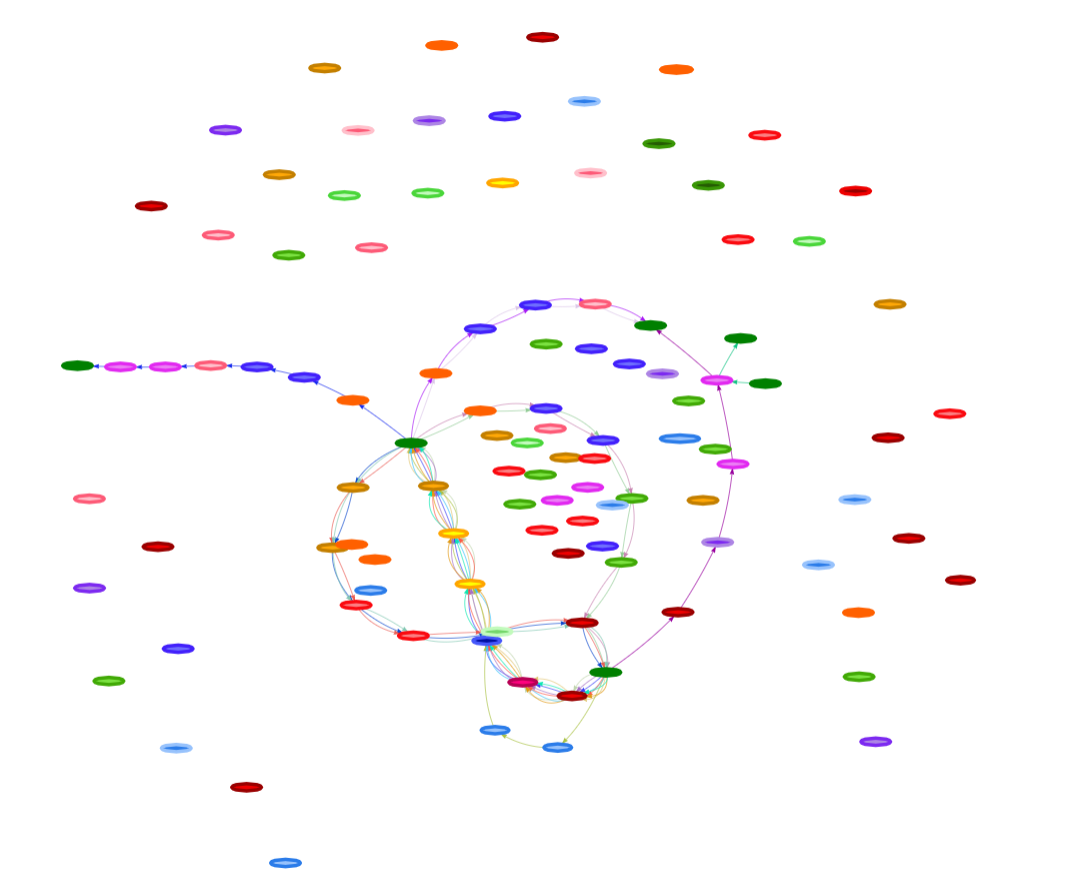
\includegraphics[width=1\textwidth]{./imagenes/resultados/resumenRepresentaion.png}
		\caption{Representación gráfica de un problema de 20 vuelos}
		\label{fig: Representación gráfica de un problema de 20 vuelos}
	\end{center}
\end{figure}

La representación gráfica muestra el resultado final del problema, es decir, se van a representar todos los vuelos a los que se les encontró solución independientemente de los instantes de tiempo en los que estuvieron en tránsito. Por tanto la representación gráfica nos permite observar qué rutas van a ser las más utilizadas.

Algunas características de la representación gráfica:
\begin{itemize}
	\item Sólo muestra los vuelos a los que se les encontró solución.
	\item Los waypoints que están ubicados en el mismo sector se marcan del mismo color (si un waypoint pertenece a más de un sector se escoge solamente el primero para simplificar).
	\item Cada vuelo tiene asignado un color para poder identificar su ruta.
	\item En las aristas del grafo representado se indica el instante de tiempo en el que un vuelo realiza ese trayecto
\end{itemize}

\begin{figure}[H]
	\begin{center}
		\centering
		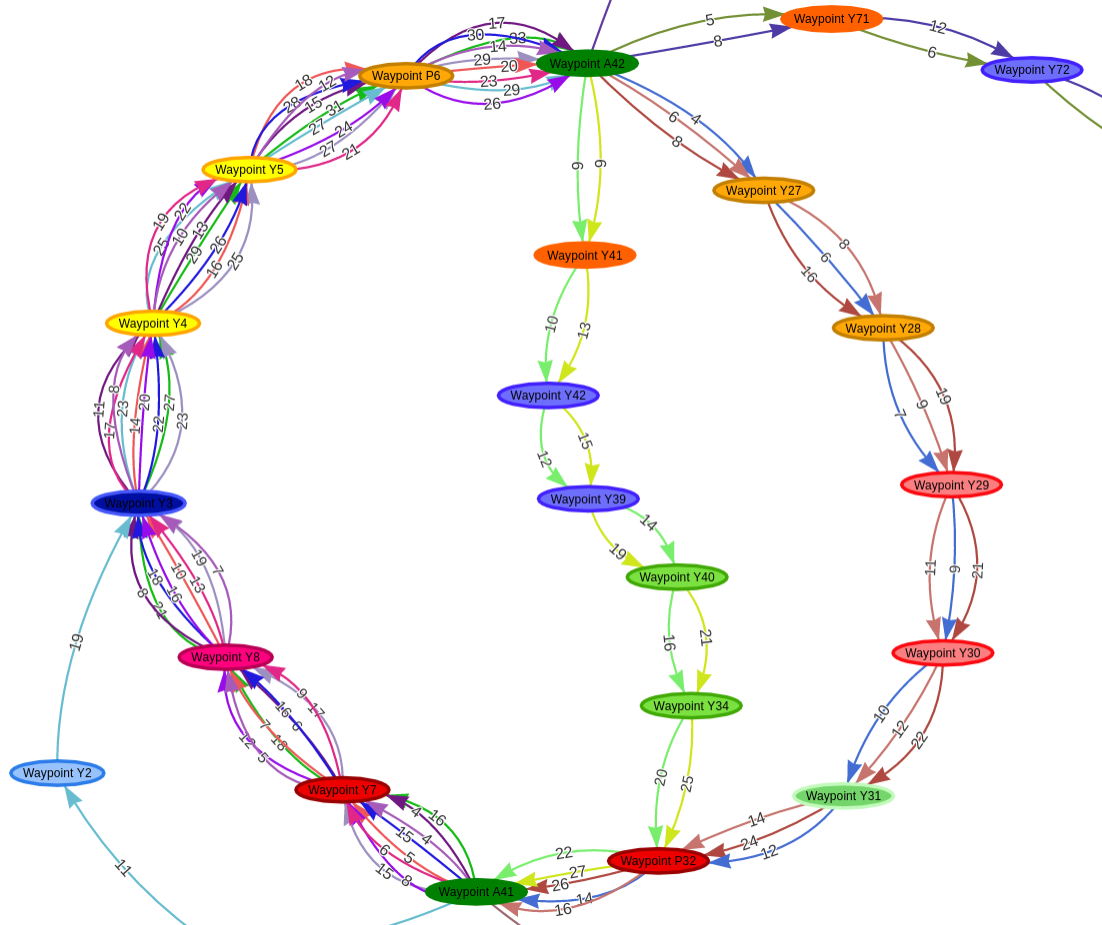
\includegraphics[width=1\textwidth]{./imagenes/resultados/representacionGrafica.png}
		\caption{Ejemplo rutas entre 2 aeropuertos}
		\label{fig: Ejemplo rutas entre 2 aeropuertos}
	\end{center}
\end{figure}

En la \autoref{fig: Ejemplo rutas entre 2 aeropuertos} se puede observar que en el trayecto entre el \textit{Aeropuerto 42} y el \textit{Aeropuerto 41} existen 2 posibles rutas: la rama derecha (más rápida y por tanto con más vuelos) y la rama entral (la ruta alternativa, ya que es más lenta).

\section{Tiempo de ejecución}
Debido al gran volumen de información se maneja el problema, comentamos brevemente el tiempo que equiere el algoritmo. Todas las pruebas han sido realizadas en un Acer Aspire-E5-573G con las siguientes características:
\begin{enumerate}
	\item Sistema operativo Ubuntu 16.04.2 LTS 64-bit.
	\item 8GB de memoria RAM.
	\item Procesador Intel Core i5-4210U CPU 1.70GHz x 4.
	\item tarjeta gráfica GeForce 920M/PCIe/SSE2.
\end{enumerate}

Los tiempos de ejecución en segundos para un problema de $N$ vuelos se resumen en la siguiente tabla y $I$ iteraciones se resumen en la \autoref{tab: Tiempos de ejecución} y en la \autoref{fig: Tiempos de ejecución del programa}:

\begin{table}[h]
	\centering
	\caption{Tiempos de ejecución en segundos }
	\label{tab: Tiempos de ejecución}
	\begin{tabular}{c|l|l|l|}
		\cline{2-4}
		& \multicolumn{1}{c|}{\textbf{N=20}} & \multicolumn{1}{c|}{\textbf{N=100}} & \multicolumn{1}{c|}{\textbf{N=800}} \\ \hline
		\multicolumn{1}{|c|}{\textbf{I=10}} &3  &21  &460  \\ \hline
		\multicolumn{1}{|c|}{\textbf{I=10}} &11  &91  &1363  \\ \hline
		\multicolumn{1}{|c|}{\textbf{I=100}} &74  &680  &9436  \\ \hline
	\end{tabular}
\end{table}


\begin{figure}[]
	\begin{center}
		\centering
		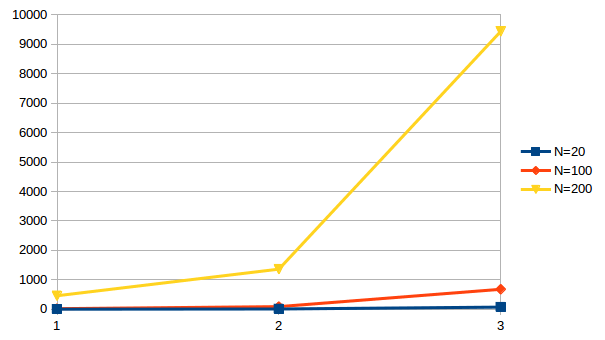
\includegraphics[width=1\textwidth]{./imagenes/resultados/tiemposejecucion.png}
		\caption{Tiempos de ejecución del programa en segundos}
		\label{fig: Tiempos de ejecución del programa}
	\end{center}
\end{figure}
